\section{Adding Spatiality}
TODO: this section may not fit: SD is the ground-truth so when coming up with total different dynamics due to adding spatiality, we open a different problem which is not really related here as they seem to counter the "real" dynamics. Also remove Randomness in Super-Sampling section

When emulating the dynamics of the SIR model using an agent-based approach the question arises what we ultimately gain from doing so when we could have generated the dynamics much quicker and smoother using the SD approach. The difference is that the agent-based approach is a stochastic one and can thus also result in "degenerated" dynamics in which the disease dies out after a few steps or even can't spread from patient zero - in this case ABS is clearly a benefit as it allows to investigate \textit{alternative futures}, something not possible with SD in which the disease will never die out prematurely when there are non-zero infected agents. \\
Another advantage of ABS over SD is that agents can be heterogeneous and make use of spatial- and/or network-information defining the neighbourhood. We can thus simulate the spread of the disease throughout a population which is laid out on a 2D grid or one can investigate spreading of the disease throughout a network of agents where some are vaccinated and others not. We provide already suitable environments to simulate these cases and show an example of spreading the disease on a 2D grid in Figure \ref{fig:sir_spatial}.  

\begin{figure*}
\begin{center}
	\begin{tabular}{c c}
		\begin{subfigure}[b]{0.4\textwidth}
			\centering
			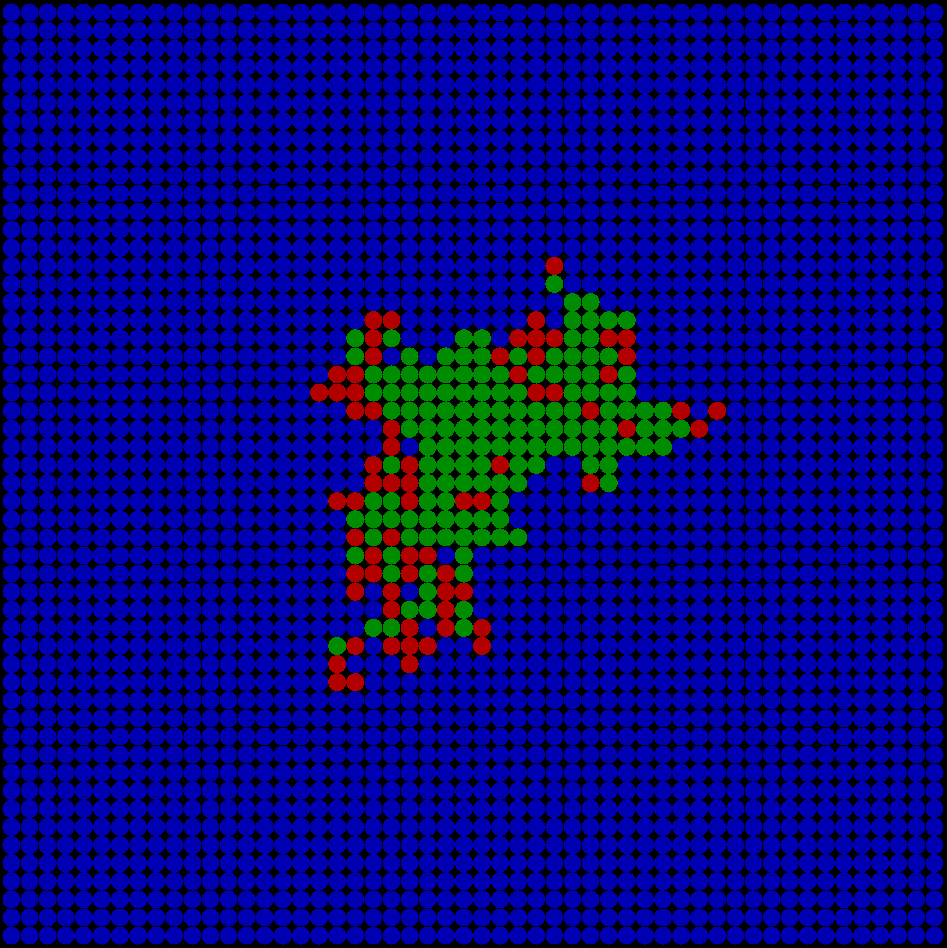
\includegraphics[width=.6\textwidth, angle=0]{./../shared/fig/spatial/SIR_spatial_52x52_92time.png}
			\caption{$t = 92$}
			\label{fig:sir_spatial_92}
		\end{subfigure}

		& 

		\begin{subfigure}[b]{0.4\textwidth}
			\centering
			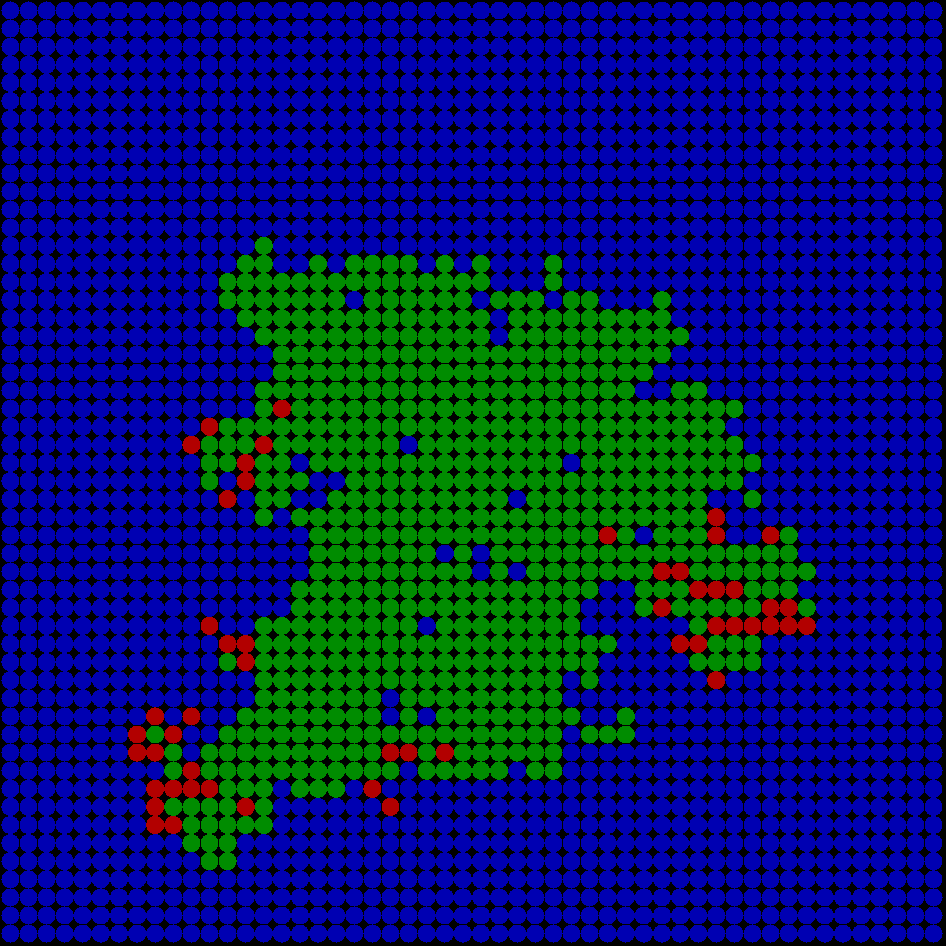
\includegraphics[width=.6\textwidth, angle=0]{./../shared/fig/spatial/SIR_spatial_52x52_200time.png}
			\caption{$t = 200$}
			\label{fig:sir_spatial_200}
		\end{subfigure}

		\\
		
		\begin{subfigure}[b]{0.4\textwidth}
			\centering
			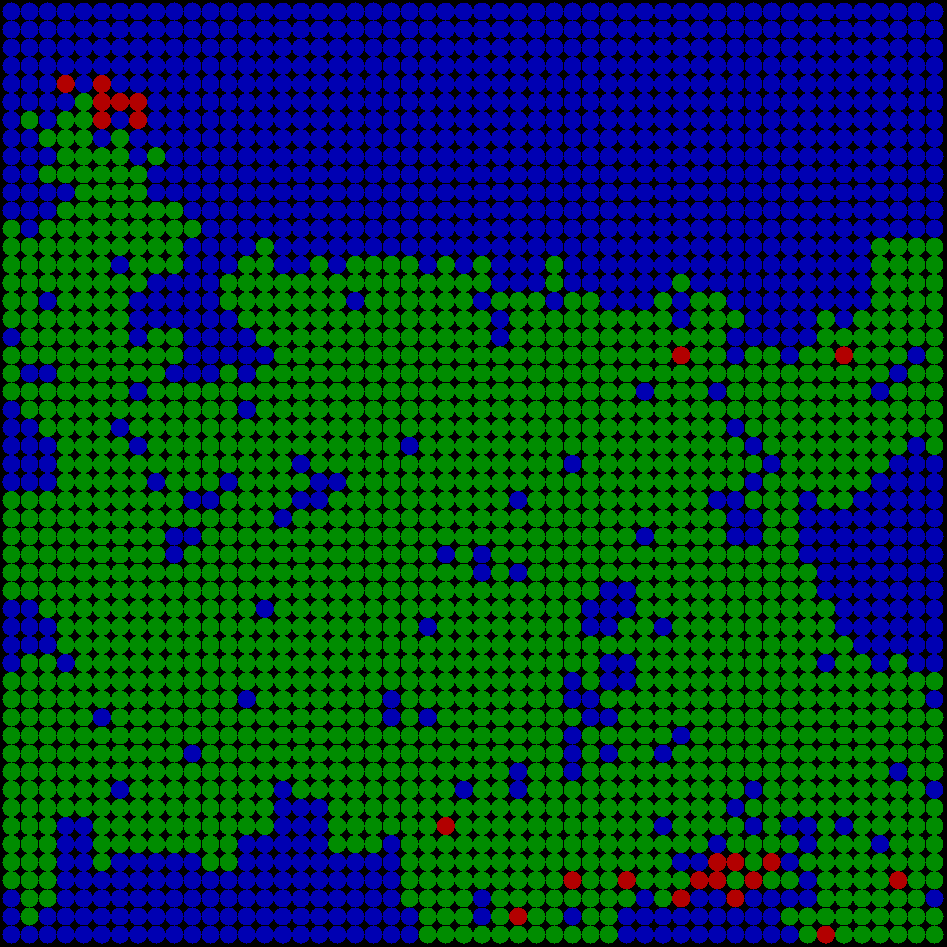
\includegraphics[width=.6\textwidth, angle=0]{./../shared/fig/spatial/SIR_spatial_52x52_440time.png}
			\caption{$t = 440$}
			\label{fig:sir_spatial_440}
		\end{subfigure}
		
		& 
		
		\begin{subfigure}[b]{0.4\textwidth}
			\centering
			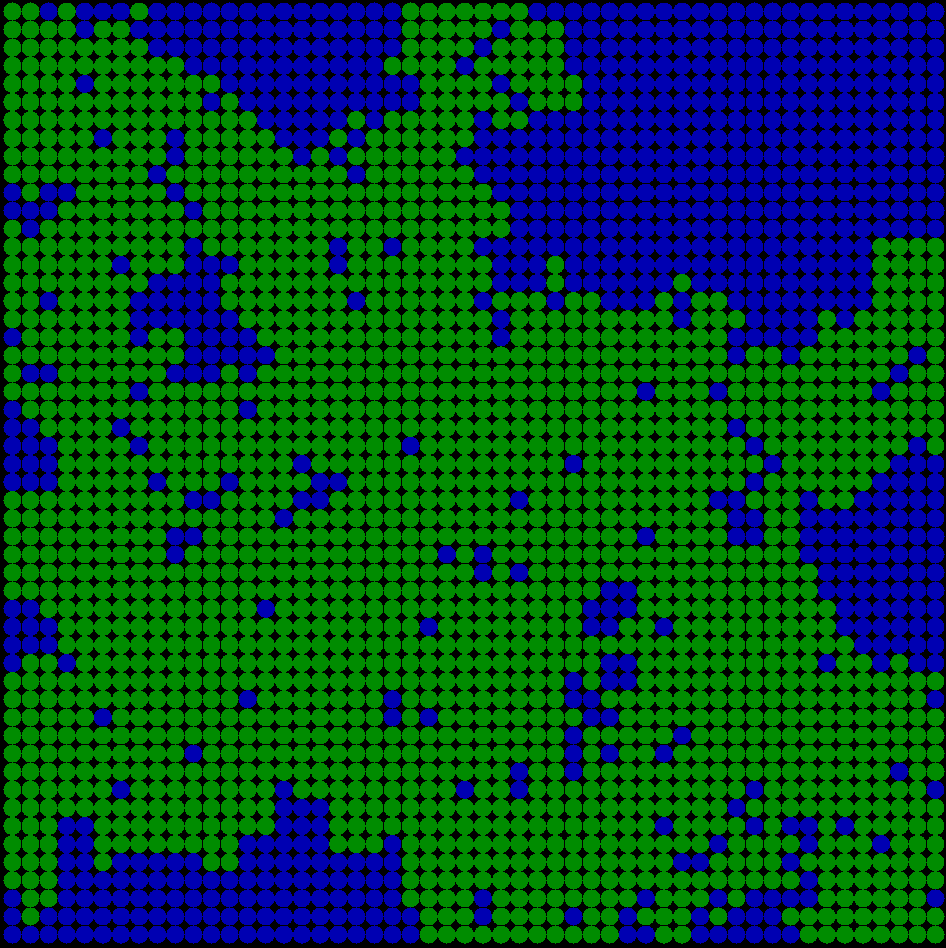
\includegraphics[width=.6\textwidth, angle=0]{./../shared/fig/spatial/SIR_spatial_52x52_873time.png}
			\caption{$t = 873$}
			\label{fig:sir_spatial_873}
		\end{subfigure}
	\end{tabular}
	
	\caption{Simulating SIR on a 52x52 grid with Moore neighbourhood using $\Delta t = 1$. Blue are susceptible, red are infected, green are recovered. The green areas act as protection as infected cannot cross the recovered border: this is particularly visible in the lower right corner of \ref{fig:sir_spatial_440} where the disease has been contained in the blue island and has no means to escape. It may seem that the few remaining infected agents in the top left corner of \ref{fig:sir_spatial_440} will die out soon but still it needs more than the already running simulation time until the disease actually dies out with the last patient recovering at center top of \ref{fig:sir_spatial_873} at $t = 873$. The dynamics of this simulation run can be seen in Figure \ref{fig:sir_spatial_dynamics}.} 
	\label{fig:sir_spatial}
\end{center}
\end{figure*}

\begin{figure}
	\centering
	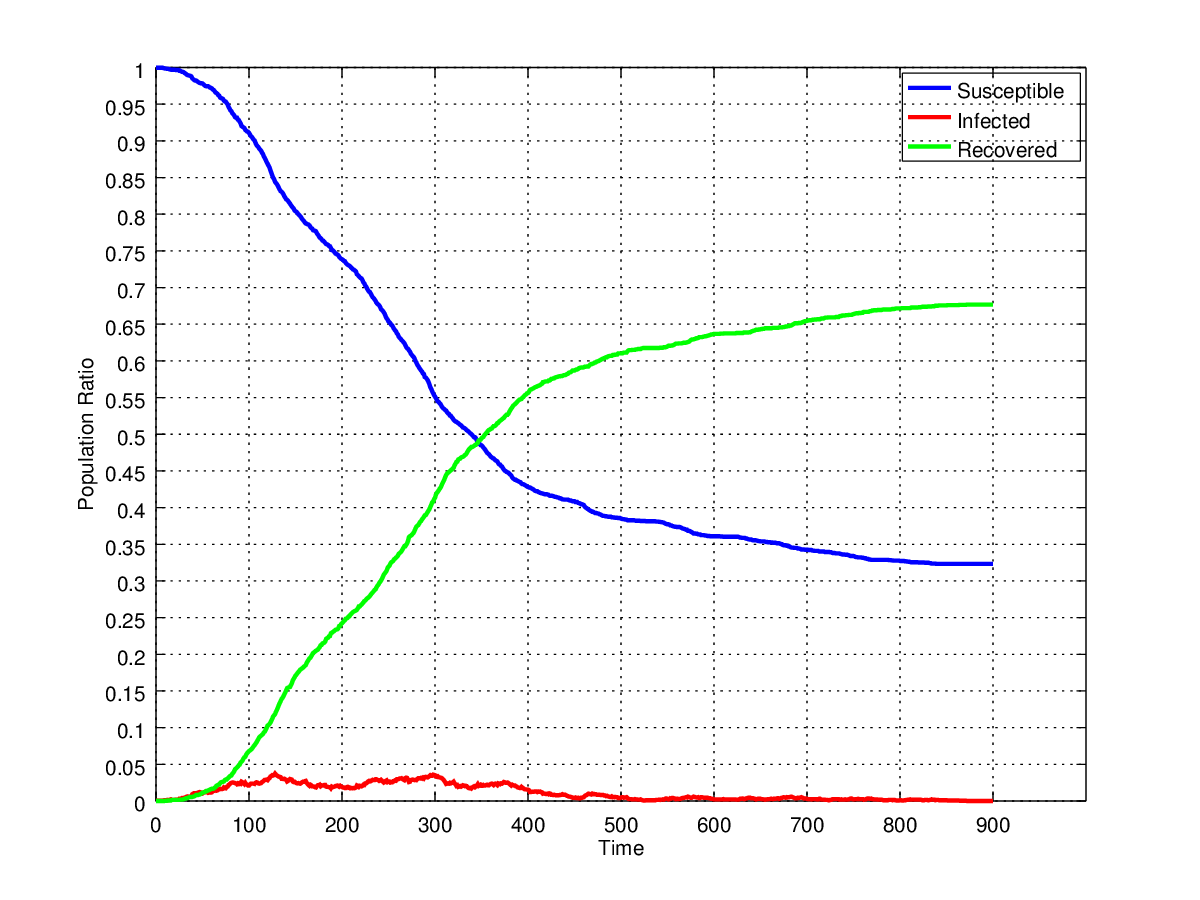
\includegraphics[width=.6\textwidth, angle=0]{./../shared/fig/spatial/SIR_spatial_dynamics_52x52_900time_1dt_parallel.png}
	\caption{Dynamics of the spatial SIR simulation from Figure \ref{fig:sir_spatial}.}
	\label{fig:sir_spatial_dynamics}
\end{figure}

Note that the dynamics of the spatial SIR simulation which are seen in Figure \ref{fig:sir_spatial_dynamics} look very different from the SD dynamics of Figure \ref{fig:sir_sd_dynamics}. This is due to a much more restricted neighbourhood which results in far fewer infected agents at a time and a lower number of recovered agents at the end of the epidemic, meaning that fewer agents got infected overall.

When using a 2D grid or network one needs to set them up in the initialization code so there is a little more work to do there but the implementation of the agents differ just in one single line, which is where the neighbourhood is picked - see line 100 of Appendix \ref{app:abs_code}. Instead of \textit{randomAgentIdMsgSource} one uses either \textit{randomNeighbourNodeMsgSource} in the case of a network or \textit{randomNeighbourCellMsgSource} in case of a 2D grid.